\section{From modified line partitions to a hypergraph}
\label{sec:deterministic-construction}

The geometric data needed for the theorem have two jobs: preserve the
intersection of point-edges after lines are split, and rule out every
cover using at most $q$ block labels. We formulate both requirements here
and prove that they suffice. The later probabilistic sections will produce
the data; all arguments in this section are deterministic and work over
any finite field.

Let $q\geq4$ be a prime power, let $A=\mathbb F_q^2$, and let
$\mathcal G$ be the set of its $q+1$ directions.  For $g\in\mathcal G$,
write $\mathcal L_g$ for the $q$ affine lines of direction $g$, and put
$\mathcal L=\bigcup_g\mathcal L_g$.  The affine line of direction $g$
through $p\in A$ is denoted by $p+g$.  We also use the projective completion
$\operatorname{PG}(2,q)$.  Thus a common projective point of affine lines
means either an ordinary point of concurrence or the point at infinity of
a parallel class.

\subsection{Merged pairs and four-point split lines}

For every direction $g$, choose two distinct lines
$M_g^0,M_g^1\in\mathcal L_g$.  Call their union the merged pair in
direction $g$, and call either of its lines a constituent.  Write
\[
 \mathcal M=\{M_g^s:g\in\mathcal G,\ s\in\{0,1\}\}.
\]
If $S\in\mathcal L_g\setminus\mathcal M$, define a simple graph on the
points of $S$: two distinct points are adjacent if they are the two
intersections of $S$ with $M_d^0,M_d^1$ for some $d\ne g$.  Several
directions may give the same adjacency; its multiplicity is irrelevant.

A tuple in direction $g$ consists of four distinct directions
$d_0,d_1,d_2,d_3\in\mathcal G\setminus\{g\}$ and four bits
$\sigma_0,\sigma_1,\sigma_2,\sigma_3\in\{0,1\}$.  Indices on the tuple
are read modulo $4$.  Define
\begin{equation}
 u_i=M_{d_i}^{\sigma_i}\cap M_{d_{i+1}}^{1-\sigma_{i+1}}.
 \label{eq:det-tuple-points}
\end{equation}
The intersections exist uniquely because consecutive generator directions
are different.  Call the tuple valid if the following conditions hold:
\begin{enumerate}
 \item Its four points are distinct and lie on one line
 $S\in\mathcal L_g\setminus\mathcal M$.
 \item Neither $\{u_0,u_2\}$ nor $\{u_1,u_3\}$ is an adjacency on $S$.
 \item Every point of $S\setminus\{u_0,u_1,u_2,u_3\}$ is adjacent to at
 most one of $u_0,u_1,u_2,u_3$.
\end{enumerate}
We call $S$ its split line and write $F_S=\{u_0,u_1,u_2,u_3\}$.  Each
consecutive pair $\{u_{i-1},u_i\}$ is adjacent: the two points lie on the
two different constituents of direction $d_i$.  Consequently the two
opposite pairs partition $F_S$, and every pair crossing that partition
shares a merged pair.

Figure~\ref{fig:cycle} records the partition and the shared merged
blocks. The conditions on opposite pairs and external points will also
control covers centered at a point of $S$.

We need two split lines in every direction. Index these requirements by
slots $(g,s)$, where $g\in\mathcal G$ and
$s\in\{1,2\}$, and choose a valid tuple in each slot. Write $S_g^s$
for its split line.
The choices are \emph{compatible} if the following conditions hold for
any two different slots:
\begin{enumerate}
 \item Neither chosen split line contains a designated point of the other
 tuple.
 \item The two sets of generator directions have intersection of size at
 most one.
 \item If the slots have the same target direction, no merged pair
 contains at least two designated points of one tuple and at least one
 designated point of the other.
\end{enumerate}
The first condition makes all chosen split lines distinct and makes their
designated point sets pairwise disjoint.  In particular, there are exactly
two split lines in each direction, both different from its two
constituents.  The second condition will be relevant to constructing such
data; the deterministic implication below uses the first and third
conditions.

\begin{figure}[htbp]
\centering
\begin{tikzpicture}[font=\small]
\node[anchor=east] at (-.2,1.1) {original class:};
\node[draw,rounded corners,minimum width=2.2cm] (ordinary) at (1.3,1.1)
 {$q-4$ other lines};
\node[draw,rounded corners,minimum width=2.2cm] (merged) at (4.1,1.1)
 {$M_g^0,\ M_g^1$};
\node[draw,rounded corners,minimum width=2.2cm] (split) at (6.9,1.1)
 {$S_g^1,\ S_g^2$};
\node[anchor=east] at (-.2,0) {new blocks:};
\node[draw,rounded corners,minimum width=2.2cm] (ordinary2) at (1.3,0)
 {$q-4$ blocks};
\node[draw,rounded corners,minimum width=2.2cm] (merged2) at (4.1,0)
 {$1$ merged block};
\node[draw,rounded corners,minimum width=2.2cm] (split2) at (6.9,0)
 {$4$ pair blocks};
\draw[-{Stealth}] (ordinary)--(ordinary2);
\draw[-{Stealth}] (merged)--(merged2);
\draw[-{Stealth}] (split)--(split2);
\end{tikzpicture}

\medskip
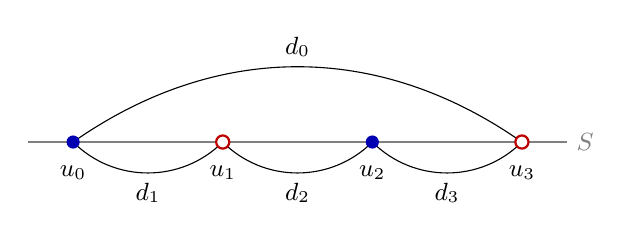
\begin{tikzpicture}[scale=.95,font=\small]
\draw[gray] (-.6,0)--(6.6,0) node[right] {$S$};
\foreach \i/\x in {0/0,1/2,2/4,3/6}{
 \coordinate (u\i) at (\x,0);
 \node[below=5pt] at (u\i) {$u_\i$};}
\draw (u0) to[bend right=45] node[below] {$d_1$} (u1);
\draw (u1) to[bend right=45] node[below] {$d_2$} (u2);
\draw (u2) to[bend right=45] node[below] {$d_3$} (u3);
\draw (u3) to[bend right=35] node[above] {$d_0$} (u0);
\foreach \i in {0,2}{\fill[blue!70!black] (u\i) circle (2.5pt);}
\foreach \i in {1,3}{\draw[red!75!black,thick,fill=white] (u\i) circle (2.5pt);}
\end{tikzpicture}
\caption{The merge and split operation gives $q+1$ blocks per direction.
Below, the four points on one split line form two opposite-pair blocks,
shown by filled and open points. An arc labelled $d_i$ means that its
endpoints lie on different constituents of the merged pair in direction
$d_i$, and hence share its block label. The arcs record this relation;
they are not affine lines. The diagram is schematic.}
\label{fig:cycle}
\end{figure}


Let $\mathcal S$ be the set of chosen split lines, and define
\begin{equation}
 \begin{split}
 D&=\mathcal S\cup\{M_g^1:g\in\mathcal G\},\\
 R_0&=A\setminus\bigcup_{\ell\in D}\ell,
 \qquad R=A\setminus\bigcup_{S\in\mathcal S}S,\\
 X&=R\cup\bigcup_{S\in\mathcal S}F_S.
 \end{split}
 \label{eq:det-core}
\end{equation}
There are exactly three lines of $D$ in each direction.  Compatibility
gives
\begin{equation}
 S\cap X=F_S\qquad(S\in\mathcal S).
 \label{eq:det-split-intersection}
\end{equation}
Indeed, $R$ contains no point of $S$, and no other designated point set
meets $S$.

The inclusion $R_0\subseteq R$ gives two retained sets with different purposes. On $R_0$, one
constituent of each merged block has disappeared, so a block cover becomes
an ordinary line cover. The larger set $R$ supplies points on the removed
constituents when we later force a cover to choose their merged blocks.
The four-point sets supply the final obstruction.

The following three properties express exactly what these sets must do.
Fix $0<\rho<1$ and an integer $B\geq0$.
\begin{description}
 \item[Occupancy.] At most $B$ constituent lines pass through any affine
 point.  Every $\ell\in\mathcal L\setminus D$ satisfies
 $|\ell\cap R_0|\geq\rho q$, and every $M_g^1$ satisfies
 $|M_g^1\cap R|\geq\rho q$.
 \item[Concentration of core covers.] If
 $C\subseteq\mathcal L\setminus D$, $|C|\leq q$, and the lines of $C$
 cover $R_0$, then at least $(1-\rho/4)q$ lines of $C$ pass through a
 common projective point.
 \item[The local condition.] For $p\in A$, define
 \[
  \mathcal S(p)=\{S\in\mathcal S:p\in S\},\qquad
  b(p)=|\mathcal S(p)|,\qquad F(p)=\bigcup_{S\in\mathcal S(p)}F_S,
 \]
 and
 \begin{equation}
 Z(p)=F(p)\cap
 \bigcup_{\substack{d\in\mathcal G,\ s\in\{0,1\}\\p\in M_d^s}}
 M_d^{1-s}.
 \label{eq:det-partner-set}
 \end{equation}
 Whenever $b(p)\geq3$, the set $F(p)$ cannot be covered by $Z(p)$ and
 at most $b(p)-1$ additional sets of the following types: sets of at most
 two points; affine lines outside $\mathcal S(p)\cup\mathcal M$; and
 merged pairs $M_d^0\cup M_d^1$, with no merged pair used more than once.
\end{description}
All these are properties of a specified finite configuration.  In
particular, none asserts that such a configuration exists.

\begin{proposition}[Deterministic reduction]
\label{prop:deterministic-reduction}
Let $q\geq4$ be a prime power.  Suppose a compatible collection of valid
tuples in $\mathbb F_q^2$ satisfies occupancy, concentration of core
covers, and the local condition with parameters $0<\rho<1$ and
$B\geq0$.  If
\begin{equation}
 \rho q>2(1+B),
 \label{eq:det-size-condition}
\end{equation}
then there is an intersecting $(q+1)$-partite $(q+1)$-uniform hypergraph
with exactly $q+1$ nonisolated vertices in each part and cover number
$q+1$.  Its edges are in bijection with the set $X$ in
\eqref{eq:det-core}.
\end{proposition}

\subsection{Partitions and intersecting edges}

We prove Proposition~\ref{prop:deterministic-reduction} in three stages:
construct the balanced partitions, reduce a small cover to one pencil,
and test the designated points against its remaining budget.

For each $g\in\mathcal G$, partition $X$ into these blocks:
\begin{itemize}
 \item $\ell\cap X$ for every regular line $\ell\in\mathcal L_g$,
 where ``regular'' excludes the two split lines and the two constituents
 in that direction;
 \item $(M_g^0\cup M_g^1)\cap X$;
 \item $\{u_0,u_2\}$ and $\{u_1,u_3\}$ for each of its two split lines,
 using that line's tuple ordering.
\end{itemize}
Distinct lines of $\mathcal L_g$ are disjoint and partition $A$, so
\eqref{eq:det-split-intersection} proves that these blocks partition $X$.
There are $(q-4)+1+4=q+1$ of them.  The split blocks have two points.
Every regular block is nonempty by the lower bound on $|\ell\cap R_0|$,
and the merged block is nonempty by the same lower bound for $M_g^0$.

Let $V_g$ consist of distinct labels for these blocks; choose disjoint
label sets for different directions.  A point $x\in X$ defines an edge
$e_x$ containing, for each $g$, the unique label of the block containing
$x$.  Thus every edge contains exactly one vertex from each of the $q+1$
parts.  Every label occurs in an edge because its block is nonempty.

For different $x,y\in X$, let $\ell$ be their joining line and let $g$
be its direction.  If $\ell$ is not a split line, then $x,y$ are in the
same regular or merged block of $V_g$.  If $\ell$ is a split line, both
points are designated by \eqref{eq:det-split-intersection}.  They either
belong to the same opposite-pair block or form consecutive positions in
its four-cycle.  In the latter case they share the merged block of the
corresponding generator direction.  Hence $e_x\cap e_y\ne\varnothing$.

Repeated edges would not affect the cover argument, but they do not
occur here.  If $e_x=e_y$ for different $x,y$, then in every direction
$h$ different from the direction of their joining line they lie on
different $h$-lines.  Their only possible common block in $V_h$ is
therefore the merged block.  The point $x$ would lie on a constituent in
each of these $q$ directions, contradicting $B<q$, which follows from
\eqref{eq:det-size-condition}.  Thus $x\mapsto e_x$ is injective.

Selecting labels covers all edges if and only if the corresponding
blocks cover $X$.  We will show that at least $q+1$ blocks are needed.
The reverse bound follows because all labels in any one part cover every
edge.

\subsection{Forcing the nonsplit members of a pencil}

We have obtained an intersecting hypergraph with the required part sizes
and no isolated vertices. Its covering number is the minimum number of
blocks covering $X$. We now use $R_0$ to locate any hypothetical small
cover, then use occupancy on $R_0$ and $R$ to force its nonsplit blocks.

Suppose that a collection $\mathcal B$ of at most $q$ labels covers $X$.
A split block misses $R_0$.  On $R_0$, a merged block is exactly
$M_g^0\cap R_0$, because $M_g^1\in D$.  Associate to each selected
regular block its line and to each selected merged block the line
$M_g^0$.  These representative lines are distinct, belong to
$\mathcal L\setminus D$, and cover $R_0$.  Concentration of core covers
provides a projective point $P$ lying on at least $(1-\rho/4)q$ selected
representatives.  Write $t$ for the number of selected labels that do not
have a representative through $P$, including all selected split labels.
Then
\begin{equation}
 t\leq\rho q/4.
 \label{eq:det-outside-pencil}
\end{equation}
We treat separately a parallel pencil and a pencil through an affine
point.

\paragraph{A point at infinity.}
Suppose $P$ is the point at infinity of direction $g$.  Every one of the
$q-3$ lines of $\mathcal L_g\setminus D$ must be a selected
representative.  Otherwise an omitted such line has at least $\rho q$
points in $R_0$, none covered by the parallel representatives through
$P$, while all remaining representatives cover at most $t$ of them.
Split blocks cover none of $R_0$, and $t<\rho q$.

The corresponding $q-3$ selected blocks cover none of the eight
designated points on the two split lines of direction $g$.  An additional
regular block covers at most one point on each of those lines, and a
split block has size two.  A merged pair of direction $g$ misses both
split lines.  A merged pair of any other direction has at most two
designated points on each split line; if it had at least three altogether,
it would have at least two on one and at least one on the other, contrary
to the third compatibility condition.  Thus every additional block
covers at most two of these eight points.  At most three labels remain
in the cover budget, so a cover is impossible.

\paragraph{An affine point.}
Now let $P=p\in A$.  We first show that for each direction $g$ such that
$p+g$ is not a split line, the selected labels must include its regular
block or, when $p+g$ is a constituent, its merged block.

If $\ell=p+g\notin D$ and its block is omitted, selected
representatives through $p$ cover at most the point $p$ on $\ell$.  All other
representatives cover at most another $t$ points there.  This contradicts
\[
 |\ell\cap R_0|\geq\rho q>1+\rho q/4\geq1+t.
\]
The strict inequality follows from \eqref{eq:det-size-condition}.

The only remaining nonsplit case is $\ell=p+g=M_g^1$.  Suppose its
merged block is omitted.  A selected regular block represented through
$p$ meets $\ell$ only possibly at $p$.  A selected merged block represented
through $p$ consists of a constituent $M_d^0$ through $p$ and its partner
$M_d^1$.  The former meets $\ell$ at $p$, and the latter contributes at
most one additional point.  None of these lines equals $\ell$, because
its own merged block was omitted.  There are at most $B$ such partners,
by the constituent multiplicity bound at $p$.  Hence all selected blocks
represented through $p$ cover at most $1+B$ points on $\ell$.  Every
other selected block covers at most two points on $\ell$: regular lines
meet it in at most one, merged pairs in at most two, and split blocks
have size two.  Occupancy on $R$ now gives the contradiction
\[
 \rho q\leq|\ell\cap R|
 \leq1+B+2t
 \leq1+B+\rho q/2
 <\rho q.
\]
This proves the claimed necessity of the block in every nonsplit
direction.

Put $b=b(p)$.  The split lines through $p$ have distinct directions,
because distinct parallel lines do not meet.  The claim therefore
requires $q+1-b$ distinct labels, leaving room for at most $b-1$ more.
It remains to check the designated points on those split lines.

\subsection{The remaining designated points}

For an affine center $p$, the nonsplit directions have forced $q+1-b$
labels, where $b=b(p)$. The possible cover therefore has at most $b-1$
labels left. The following cases show that the designated points on its
$b$ split lines cannot be covered within that budget.

If $b=0$, the required $q+1$ labels already exceed the budget.  If $b=1$,
write $S$ for the unique split line through $p$.  Exactly $q$ labels are
required, so no additional label is available.  On $F_S$ their blocks
can cover only $p$ itself, when $p\in F_S$, and points adjacent to $p$
on $S$: regular lines through $p$ supply only $p$, and a merged pair
through $p$ supplies only its partner intersection.  If $p=u_i$ is
designated, its opposite point $u_{i+2}$ is not adjacent to it and is
missed.  If $p\notin F_S$, validity allows at most one designated point
adjacent to $p$.  In either case $F_S$ is not covered.

Suppose now that $b\geq2$.  Compatibility implies that $p$ is not
designated on any split line through it: otherwise that point would lie
on a second chosen split line.  The designated sets on these lines are
pairwise disjoint, so $|F(p)|=4b$.  A required regular block through $p$
meets any such split line only at $p$ and therefore misses its designated
points.  A required merged block has one constituent through $p$ and
can cover designated points only with its partner.  Thus the required
blocks cover a subset of $Z(p)$.

For each $S\in\mathcal S(p)$, every point in $Z(p)\cap F_S$ is adjacent
to the external point $p$ in the graph on $S$.  Validity gives
$|Z(p)\cap F_S|\leq1$, and consequently
\begin{equation}
 |Z(p)|\leq b.
 \label{eq:det-partner-count}
\end{equation}
If $b=2$, at most one additional block is available.  A regular line
meets the two split lines in at most two points, a merged pair in at most
four, and a split block has two points.  Hence this extra block together
with $Z(p)$ covers at most $4+2<8=|F(p)|$ points.

Finally, let $b\geq3$.  Each of the at most $b-1$ additional labels is
represented on $F(p)$ by one of the sets allowed in the local condition:
a split block has two points, a regular line is outside
$\mathcal S(p)\cup\mathcal M$, and a merged block is contained in its
merged pair.  No merged pair is repeated because it has only one label.
The local condition therefore rules out covering $F(p)$.  This is the
last possible case, completing the proof of
Proposition~\ref{prop:deterministic-reduction}.

\begin{remark}
For the multiplicity bound $B=\lceil\log q\rceil$ used in the
probabilistic construction, it is enough to require explicitly
$q\geq4$ and $\rho q>2(1+\lceil\log q\rceil)$.  Every fixed
$\rho>0$ satisfies this inequality for all sufficiently large $q$.
Primality is not used in the deterministic reduction; any restriction
to prime orders must come from establishing the finite configuration
properties.
\end{remark}
